%%%%%%%%%%%%%%%%%%%%%%%%%%%%%%%%%%%%%%%%%
% Thesis 
% LaTeX Template
% Version 1.2 (29/7/12)
%
% This template has been downloaded from:
% http://www.latextemplates.com
%
% Original authors:
% Steven Gunn 
% http://users.ecs.soton.ac.uk/srg/softwaretools/document/templates/
% and
% Sunil Patel
% http://www.sunilpatel.co.uk/thesis-template/
%
% License:
% CC BY-NC-SA 3.0 (http://creativecommons.org/licenses/by-nc-sa/3.0/)
%
% Note:
% Make sure to edit document variables in the Thesis.cls file
%
%%%%%%%%%%%%%%%%%%%%%%%%%%%%%%%%%%%%%%%%%

%-----------------------------------------------------------------------------
%	PACKAGES AND OTHER DOCUMENT CONFIGURATIONS
%-----------------------------------------------------------------------------

\documentclass[11pt,a4paper, wide, twoside]{IIBproject}

\graphicspath{{./Pictures/}} % Specifies the directory where pictures are stored

\usepackage[round, sort&compress]{natbib} % Use the natbib 
  %reference package - read up on this to edit the reference style; 
  %if you want text (e.g. Smith et al., 2012) for the in-text references 
  %(instead of numbers), remove 'numbers' 

\usepackage{caption}
\captionsetup{margin={15pt},parskip=10pt,format=hang,indention=-.8cm}

\usepackage{type1cm}
\usepackage{lettrine}

\usepackage{tikz}
\usetikzlibrary{matrix,shapes,arrows,patterns,snakes}

\tikzstyle{block} = [draw, fill=blue!20, rectangle, minimum height=3em, 
                      minimum width=6em]
\tikzstyle{sum} = [draw, fill=blue!20, circle, node distance=1cm]
\tikzstyle{input} = [coordinate]
\tikzstyle{output} = [coordinate]
\tikzstyle{branch}=[fill,shape=circle,minimum size=3pt,inner sep=0pt]
\tikzstyle{label} = [text width=7em, text centered, font=\itshape]

\tikzstyle{key} = [draw, circle, fill=black, minimum width=5mm, inner sep=0pt,
  minimum height=5mm, text centered, text=white,font=\small\bfseries]

%for HMM diagram
\tikzstyle{match} = [draw, fill=blue!20, rectangle, inner sep=0pt, 
                    minimum height=1cm, minimum width=1cm, font=\footnotesize]
\tikzstyle{insert} = [draw, fill=yellow!40, diamond, inner sep=0pt,  
                    minimum height=1cm, minimum width=1cm, font=\footnotesize]
\tikzstyle{delete} = [draw, fill=red!20, circle, inner sep=0pt,  
                    minimum height=1cm, minimum width=1cm, font=\footnotesize]

%\usepackage[plainpages=false]{hyperref}
%\hypersetup{urlcolor=black, colorlinks=true} % Colors hyperlinks in blue - change to black if annoying

\begin{document}

\setstretch{1.5}

\pagenumbering{roman}
% PDF meta-data
%\hypersetup{pdftitle={\ttitle}}
%\hypersetup{pdfsubject=\subjectname}
%\hypersetup{pdfauthor=\authornames}
%\hypersetup{pdfkeywords=\keywordnames}

%----------------------------------------------------------------------------------------
%	TITLE PAGE
%----------------------------------------------------------------------------------------

% Title Page
\author{Haydn \textsc{King} (JE)}
\name{Haydn King}
\title{A Cross-Genome Study of the Pentatricopeptide Repeat Protein}
\projectgroup{F}
\maketitle

%----------------------------------------------------------------------------------------
%	ABSTRACT PAGE
%----------------------------------------------------------------------------------------
\setcounter{page}{1}

\abstract{

The Thesis Abstract is written here (and usually kept to just this page). 
The page is kept centered vertically so can expand into the blank space above 
the title too\ldots

}

\clearpage % Start a new page

%----------------------------------------------------------------------------------------
%	LIST OF CONTENTS/FIGURES/TABLES PAGES
%----------------------------------------------------------------------------------------

\setcounter{tocdepth}{1}
\tableofcontents % Write out the Table of Contents

\clearpage % Start a new page

%----------------------------------------------------------------------------------------
%	CONTENT - CHAPTERS
%----------------------------------------------------------------------------------------

\pagestyle{mainstyle}
\pagenumbering{arabic}

% Include the chapters of the thesis as separate files from the Chapters folder
% Uncomment the lines as you write the chapters


\chapter{Introduction}
\label{chap:Introduction} 

\section{Molecular Biology}
\label{sec:MolecularBiology}

Molecular biology is the study of the molecular basis of biology.
It is mostly concerned with the understanding of the systems and processes
that occur within a living cell.
Naturally, the field overlaps considerably with other areas, 
such as genetics (the study of genes and heredity) and biochemistry (the study
of the chemical processes of life).

While the field itself is rather broad, much of it is underpinned by what is
referred to as the central dogma of molecular biology -- 
DNA makes RNA makes proteins.
This central dogma describes the flow of information within a cell and the
processes and control mechanisms which regulate this process.
Naturally, many of these processes are highly complicated and poorly
understood, but much progress has been made since the discovery of DNA in the
1950s to understand these processes.
Figure~\ref{fig:processes} shows the most important of these processes and how
they convert between the three most important classes of molecules in the cell.

\begin{figure}
  \centering
  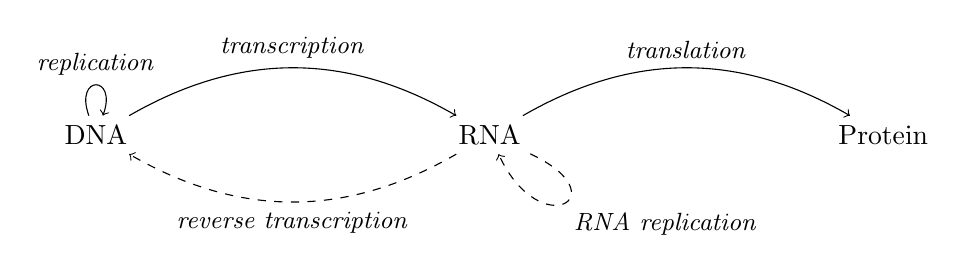
\begin{tikzpicture}[node distance=5cm, auto]
    \node (D) {DNA};
    \node (R) [right of=D] {RNA};
    \node (P) [right of=R] {Protein};
    \draw[->, bend left] (D) to node {\small \textit{transcription}} (R);
    \draw[->, bend left] (R) to node {\small \textit{translation}} (P);
    \draw[->] (D) to [out=110,in=70,looseness=8] 
                node {\small\textit{replication}} (D);

    \draw[->, dashed, bend left] 
      (R) to node {\small \textit{reverse transcription}} (D);
    \draw[->, dashed] (R) to [out=335,in=295,looseness=8] 
                node {\small\textit{RNA replication}} (R);
  \end{tikzpicture}
  \caption{The main processes in molecular biology. The three most common are
    shown using solid lines while two important but less common processes are
    shown in dotted lines.
    \label{fig:processes}}
\end{figure}

Molecules of DNA are the cell's long term storage mechanism -- recent research
estimates the half-life of DNA to be 521 years\cite{DNAhalflife}.
DNA molecules are long sequences of simple nucleotides which encode all the
genetic information of the cell.
Each nucleotide contains a nucleobase which is either Adenine, Guanine,
Thymine or Cytosine (A,G,T or C) and it is the sequence of so called bases which
determines the information content of the molecule.
DNA is double-stranded -- each base in the chain forms a hydrogen bond with a
base from a complementary chain of DNA.
These strands are coiled around each other into DNA's characteristic 
double-helix structure.

The data stored in DNA is read by a molecule called RNA polymerase which 
produces an RNA copy of a section of the DNA in a process called
\textit{transcription}.
RNA is similar to DNA, but is short-lived (lasting minutes to hours) and so the
RNA copy is referred to as a messenger-RNA (mRNA) molecule.
This message is then read by a ribosome, a molecule which translates the mRNA 
into a protein, a process referred to as \textit{translation}.
Proteins a chain of amino acids which fold into a very specific shape and 
perform many important functions within the cell.
The region of DNA which encodes a particular protein is called a \textit{gene}.

The processes of transcription and translation through which genes are 
expressed (produce proteins) are typically very tightly
controlled by the cell, as this is the main way of influencing the levels of
various proteins within the cell and thus the cell's overall activity.

\subsection{Transcription}
\label{sec:transcription}

Both DNA and RNA have an alphabet of four symbols and so during transcription,
DNA's alphabet, $\{A,C,G,T\}$, is mapped one-to-one to that
of RNA, $\{A,C,G,U\}$, where thymine is replaced with uracil.
Transcription is clearly bijective, and indeed a less common process called
reverse-transcription performs the inverse mapping from RNA to DNA.

Transcription does not act on an entire DNA strand at once but instead
transcribes a small region of the DNA called a transcription unit, which
contains one or many genes.
These units are marked by promoters which are regions of DNA upstream
of the transcription unit that initiate transcription by causing RNA polymerase
to bind.
Control is commonly achieved by modulating promoter activity.


%Proteins are a sequence of amino acids, where each acid comes from an alphabet
%of 20 amino acids.
%Each acid is coded for by 3 base pairs of RNA, which are referred to
%collectively as a codon.
%Since there are $4^3$ possible codons and only 20 amino acids, the code is
%over complete -- several different codons map to the same amino acid.
%As well as coding for amino acids, three special codons (UAG, UAA and UGA) are
%known as stop codons as they terminate the translation of the protein.
%
%
%
%Ribosomes bind to the mRNA, reading the gene and creating the appropriate
%protein before detaching from the mRNA.
%mRNA is more fragile than DNA but is also targeted by exonucleases, a class of
%enzyme which degrade RNA molecules, preventing the production of more protein.
%Similar processes exist to degrade proteins over time, recycling their amino
%acids to form new proteins.
%These degradation processes mean that a gene must continue to be transcribed at
%a constant rate for the concentration of its protein to remain constant.
%


\section{Synthetic Biology}
\label{sec:synbio}

Synthetic biology is a relatively new
engineering discipline with the goal of applying standard engineering techniques
such as standardisation, characterisation and encapsulation of function to 
biology.
Synbio aims to use these design principles to combine existing phenomena to 
build new, artificial forms of life.
The field is often confused with its spiritual predecessor, genetic 
engineering, which although similar in some respects does not design new
organisms, but tinkers with existing ones without trying to understand the
underlying principals.

Synbio is often referred to as programming, but with DNA instead of computer
code.
An example project which captures this idea is Tabor's bacterial edge
detector\cite{edgeDetector}.
Bacteria were programmed to produce a colourless chemical messenger in the 
absence of light and to produce a dark pigment in the presence of light and the
chemical messenger.
When a film of these bacteria is exposed to a pattern of light and dark, the
messenger diffuses out from the dark regions and into the light, where it
stimulates the production of the pigment, leading to an edge detection effect.

While this and other such simple demonstrations show some of the potential 
of synbio, they lack immediate application and are somewhat limited.
A major problem in expanding this work is the lack of targeted reporter
molecules.
In the edge-detector example, two molecular signals are produced when light is 
not present -- AHL, a cell-to-cell signalling molecule and cI, a
transcriptional repressor molecule.
Both AHL and cI are known to affect the promoter $P_{lux-\lambda}$; while AHL 
stimulates expression, cI strongly represses it.
With expression of the dark pigment being driven by $P_{lux-\lambda}$, 
both light and AHL are required to cause the pigment to be produced.

The effect of the molecules AHL and cI on $P_{lux-\lambda}$ is one of a small
but growing number of well understood control motifs.
Since reusing the same promoter/signal in the same cell is impossible due to 
cross-talk, there are simply not enough signalling modalities available to
perform more complex calculations within the cell.
Indeed, it is often the case that signalling molecules have multiple functions
within the cell such that changing the concentration of one molecule to suit
our goals may cause a seemingly unrelated area of the cell's metabolism to
malfunction with undesirable consequences.

A more applicable synbio project was the effort to produce 
artemisinin (the most effective known anti-malarial) in a cheaper and more 
scalable way.
Artemisinin is found naturally in sweet wormwood, but it is slow and expensive
to extract directly from the plant and chemical synthesis is also an expensive
and laborious process.
Synthetic biologists were able to extract the metabolic pathway responsible for
the biosynthesis of artemisinic acid (a natural precursor) and insert it into 
yeast\cite{yeast}.
Artemisinin produced in this manner has yet to be approved for sale, but it is
hoped that it should be available at some point during 2013, at a considerably
lower price than any other method of production.

The major limiting factor in this project was yield.
In order to produce a useful amount of the drug, the pathway involved had to be
up-regulated, which led to a difficult balance -- too little and very little
artemisinic acid would be produced, too high and too much of the cell's
energy would be used, causing the cells to grow slowly if at all.
As well as this, growing yeast on an industrial scale is relatively expensive.
It is desirable therefore search for host platforms which are better suited to
biosynthesis than yeast, in order to maximise the yield to cost ratio.

Chloroplasts are a major centre for biosynthesis in plants as they perform
photosynthesis to provide energy for the plant.
The result of an ancient symbiosis, up to 1000 of these primitive cells can be 
found within each plant cell, where they make an excellent target for synbio.
They are similar to previous synbio hosts, but with access to the more
sophisticated plant cell machinery and superb potential for biosynthesis.
The native enzyme RuBisCO is so abundant in the chloroplasts that it 
can be up to 50\% of overall soluble leaf protein.
Achieving anything remotely close to this figure in a project such as the
production of artemisinin would help reduce the vast number of people who die 
of this treatable disease each year (roughly 2,000 deaths a day in 2010
\cite{malaria}).

\subsection{The PPR Protein}

Brief introduciton to what a PPR protein is and why they are interesting, 
reference Section \ref{sec:PPR} heavily.



\chapter{Automating PPR discovery} 
\label{chap:methods}

\lettrine{M}{ost} 
sequenced genomes are also annotated with information about the genes they
encode a specific locations.
These annotations are usually very helpful when navigating the genome as many
are the result of empirical study.
The majority of PPRs have not been studied in detail, however, and thus their
annotation is often unreliable and certainly doesn't contain information about 
the PPR motifs found within the proteins.

For this reason it was necessary to develop routines for discovering and
extracting PPR proteins from unannotated genomes, using a hidden Markov model
of the characteristic repeat motifs to find likely targets.
Having identified PPRs, we would like to be able to predict their binding
locations within organelles.

The development of algorithms to achieve these things is discussed in this
chapter.

\section{pyHMMER}
\label{ssec:pyHMMER}

The HMMER suite provides all of the basic algorithms required in order to
perform an HMM search on a target amino acid sequence, but it does have some
limitations.

The first is that it is a command line program and does not have bindings to
any programming language.
HMMER reads inputs from files, and writes out tabular output data to file which
would be very time consuming to parse by hand.

HMMER cannot translate sequences on the fly -- is can only compare a protein 
model with a protein target, and so the genome must be translated before 
HMMER is invoked.
There are a total of six possible reading frames (3 forwards and 3 backwards, 
due to the 3:1 nature of translation) and the genome must be searched in each
of these six frames.

HMMER is not commercial software and is developed by a group of scientists at
the Howard Hughes Medical Institute (HHMI) under an open licence for research
purposes.
As such, it contains a number of minor bugs which are not fatal to the
software's functionality, but can sometimes cause problems
under particular circumstances.
The most problematic of these causes enormous
memory usage (over 20GB\footnote{One particular instance of this error is due
to an unsigned integer wrap-around which causes significantly more memory to be
requested from the operating system than could possibly be needed}) and
prevents the program from completing.

In order to overcome these issues, a python wrapper for HMMER called
pyHMMER was designed and written as part of this project.
Python was chosen as the main language mainly because of its
excellent library support -- for example the biopython library solved many of 
the difficulties when working with biological sequences without extra effort.

pyHMMER does not implement all the features available in HMMER, but rather it
implements those which were most vital to this project.
Its main features are -
\begin{itemize}
  \item Read and write \emph{.hmm} files, HMMER's custom file format for
    storing HMMs
  \item Execute searches using 
    \emph{hmmsearch} and \emph{jackhmmer}, accepting all valid command line
    arguments and returning their output as biopython objects, 
    handling the creation and removal of all the necessary 
    temporary files automatically
  \item Seamlessly perform six-frame translations on the fly (implemented in C
    for best performance) and correctly map the location of each match to the 
    original target alphabet
  \item Automatically terminate HMMER processes which attempt to allocate more
    memory than the system can sensibly be expected to 
    provide\footnote{Linux only} and then call
    HMMER sequentially with subsections of the target, automatically mapping
    all matches back to the original target
  \item Fully unit-tested with python's \emph{unittest} framework
\end{itemize}
pyHMMER has been developed under an open-source licence and is freely available
from \emph{https://github.com/haydnKing/pyHMMER}, although all code used in
this project was written by myself.


\section{Automated PPR Detection and Extraction}
\label{sec:ppr_extraction}

Several algorithms were developed and compared in order to extract PPRs from
unannotated genomes.
The results of each algorithm were compared with experimentally validated PPRs
and the best chosen.

Before development could begin, a HMM of the PPR repeat motif was required.
There are four such models available in
Pfam\footnote{http://pfam.sanger.ac.uk/search/keyword?query=PPR}, and each one
was tested on known PPRs in order to discover which model worked best when
searching for motifs.
It was found the PPR\_3 model is most sensitive to the motifs, yet still
returns few false positives.

Armed with this model, the final algorithm for discovering PPRs proceeds as
follows for each chromosome within the genome
\begin{enumerate}
  \item \label{alg:first_pass}
    Perform a HMM search on the whole sequence. This will discover the most
    obvious motifs only
  \item \label{alg:grouping}
    Cluster the motifs into groups such that members of the same group are on
    the same strand and are within a certain distance of each other
  \item \label{alg:envelopes} 
    For each group, extract and `envelope' region containing each motif in the
    group along with large margins either side. 
  \item \label{alg:second_pass}
    Search each envelope region for PPR motifs. This search is more
    focussed than the previous one and will reveal more motifs than previously.
    Discard any envelopes which contain only one motif.
  \item Starting from the first position of the first motif, search backwards
    one codon at a time until a start codon (`ATG') is reached
  \item Starting from the last position in the final motif, search forwards one
    codon at a time until a stop codon is reached (`TGA', `TAG' or `TAA').
    Extract the putative PPR from between the start and stop codon
  \item \label{alg:overlap}
    Check for PPRs which overlap. 
    Each set of overlapping proteins should be removed and a new, larger
    envelope extracted. The algorithm then continues again from step
    \ref{alg:second_pass} with the new envelopes
  \item \label{alg:large_proteins}
    Check for PPRs where the motifs have filled the envelopes -- i.e. ones
    which are missing a start or a stop codon due to not having searched far
    enough. Extract larger envelopes for these proteins and continue from step
    \ref{alg:second_pass}
  \item \label{alg:reluctance}
    Search each protein for gaps between motifs which are the correct size
    to fit a PPR motif. Search these regions specifically, increasing HMMER's
    sensitivity to look for reluctant PPR
    motifs. Also search the beginning and the end of the protein in this way
  \item \label{alg:remove_gaps}
    Search each protein for small (2/3 codon) gaps between the motifs and
    move the end position of the previous motif in order to fill these gaps.
    This allows the motifs to be classified as P, L or S
  \item \label{alg:classification} 
    Classify the proteins depending on which types of motifs they contain.
    Extract the protein sequence of each tail sequence and classify it using
    \emph{jackhmmer} to search for the known consensus sequences for E, E+ and
    DYW motifs
  \item \label{alg:subcellular_location}
    Predict each protein's sub-cellular location using the \emph{targetP}
    program
\end{enumerate}
A brief discussion of the rationale and implementation of the most important 
steps follows.

The reason why the motifs found in step \ref{alg:first_pass} cannot simply be
accepted is due to the degenerate nature of the motifs.
It would be possible to decrease HMMER's reporting threshold as to return all
possible motifs but since the search space is large and the model accepts a
wide range of sequences, there would be a large number of false positives.
By using default values for these thresholds there is unlikely to be a problem 
as HMMER is designed to show the most probable matches and only a few of
the possible false positives.
The presence of a few false positives at this stage is not an issue because the
chance of finding several false positives immediately adjacent to each other 
(as would be required to pass the later stages of the algorithm) is highly 
unlikely.

Having found the most obvious motifs, step \ref{alg:grouping} groups motifs
which are believed to belong to the same protein.
Initially this was restricted to motifs which were in the same reading frame
(i.e. the gaps between start of each motif were multiples of three), 
but this was later expanded to all motifs on the same strand, as introns 
(see sections \ref{sec:transcription} and \ref{sec:translation}) 
are known to be present in some PPR motifs.
Experiment showed that grouping motifs which were within $1500bp$ of each other
gave good results.
Grouping was implemented by first sorting the motifs into ascending order and 
then searching through linearly giving a cost of $O(n \log n)$ rather than the 
cost of $O(n^2)$ required for exhaustively comparing each motif.

Envelopes are then extracted from these groups in step \ref{alg:envelopes}.
The term `envelope' is borrowed from HMMER's output and refers to the fact that
we expect there to be a PPR somewhere within this region, but we are not sure
where exactly.
For envelopes on the reverse strand, the sequence is extracted such that it
reads in the 5' to 3' direction on that strand.
It is important to maintain a record of where in the target sequence the
envelope came from, as this information may be required later in the algorithm.
A margin of $1000bp$ either side of the group was found to give good results.

The search space in step \ref{alg:second_pass} is several orders of magnitude 
smaller than the first pass and so the chances of finding multiple high-scoring 
matches by chance are negligible.
Shortening the target in this way effectively moves HMMER's baseline for
scoring matches such that lower scoring matches which would previously have 
been written off as noise are now treated as legitimate matches.

Steps \ref{alg:overlap} and \ref{alg:large_proteins} effectively correct for
situations where the parameter values chosen for grouping and envelope
extraction do not perform well.
For example, if step \ref{alg:first_pass} detects the first and last motifs
from a particularly long PPR then these will be treated as belonging to 
separate proteins up until this point.
Similarly, if only one motif was detected then the size of the actual protein
may be larger than the envelope which is extracted.

These two steps introduce loops into the algorithm and thus introduce the
worrying possibility of an infinite loop preventing the algorithm from
completing.
In the case of step \ref{alg:overlap} this cannot happen as for each
iteration of the loop the number of putative proteins is half that of the
previous loop, meaning that no infinite loop is possible.
An infinite loop is also impossible in \ref{alg:large_proteins}, as the growth
of the envelope is limited by the size of the search query. 
However, since each loop iteration is expensive and adds only a constant 
length to the envelope this could take quite some time in the worst case.
To protect from this, a large upper bound was placed on the maximum length of 
a protein.

Proteins which are input to step \ref{alg:reluctance} often contain gaps of
around 35 amino acids -- the correct size for a repeat motif -- and comparison
with known proteins shows that a motif should indeed be placed in this region.
These motifs can be found by searching these regions with a lower reporting
threshold than the default.
A plausible explanation of these poorly conserved motifs is that the presence of
relatively well conserved (and thus well folded) regions on either side of the
degenerate motif increases its tendency to fold correctly.
However it could also be the case that these regions simply represent a gap in
the recognition chain (where any base would be accepted) or an intron; more
empirical results are needed in order to determine this in every case.
Setting each of the parameters \emph{F1}, \emph{F2} and \emph{F3} to $0.5$ 
gave a reasonable trade-off between finding likely reclusive motifs and 
rejecting random sequences.

Studies such as \citet{Lurin2004} have shown that tandem PPR repeat motifs tend
not to have small gaps between them.
Since pyHMMER returns the location of the HMMER model, each match is the same
length as the model.
This is corrected for in step \ref{alg:remove_gaps}, such that the motifs can
be classified as type P (length~$=$~35aa), L (length~$>$~35aa) or 
S (length~$<$~35aa).

The final two stages classify the extracted proteins depending on their type
and sub-cellular targeting.
Step \ref{alg:classification} makes use of the \emph{jackhmmer} program which
iteratively constructs HMM models of a consensus sequence based on a target
sequence and is supported by pyHMMER.
The final step uses \emph{targetP}, a well respected prediction algorithm for
sub-cellular localisation\citep{targetP}.

\section{Predicting PPR Binding regions}
\label{sec:ppr_binding_prediction}

Given an extracted and well annotated PPR protein, predicting the RNA footprint
to which is binds is not straightforward.
In the case of TALEs (section \ref{sec:intro_binding}), a well known mapping
exists between the amino acids at specific locations within the repeat and the
preferred DNA base of that repeat.
Unfortunately, such a mapping has yet to be confirmed for the PPR family,
although two main suggestions have been made, by \citet{Barkan2012} and by
\citet{Yagi2013}.

Since neither the structure of of the PPR motif or of a PPR-RNA complex
has been solved, the only method to elucidate the rules governing binding
preferences is by looking for statistical dependencies between the amino-acid
sequence and RNA footprint of known PPR-RNA pairs.
This is the strategy used by both papers mentioned above and so they lead to
similar results.
The papers each provide methodologies to convert each PPR motif into a
distribution over each the symbols in RNA, $\{A,C,G,U\}$.

The next two sections outline methods for discovering likely binding sites
in a particular target given a sequence of such distributions.

\subsection{Profile Hidden Markov Models}
\label{sec:hmm_binding}

The first method which was tested was using pHMMs, as this would allow the use
of HMMER's advanced searching algorithms.
This seems a simple task -- the probabilities given at each motif give the
emission probabilities at each node, insert probabilities can be uniform and
the transition probabilities can be determined empirically.

The first issue which arises is that pHMM models which are used for searching
with HMMER must be normalised in order to make score calculations.
This involves estimating the parameters of the distribution of model scores 
for random sequences.
A program called \emph{hmmsim} exists in the HMMER package for just 
this purpose, however the program is not a mainstream part of the HMMER package
and is present more as a tool for testing HMMER's internals rather than use by
the end user.
As a result, it is not as stable as other HMMER tools and has not been tested
with all possible use cases.
Unfortunately, one particular unanticipated use case is the normalisation of a
DNA model -- \emph{hmmsim} is hard-coded to accept only protein models as this
is HMMER's primary use case.

This problem was circumvented by writing the model as a protein model by
expanding the probabilities of each of the four bases to those of the 20 
amino acids (i.e. the first 5 amino acids corresponding to an `A' etc\ldots).
However models which had been normalised in this way did not prove to be
effective when searching large sequences even when a known high scoring
sequence was inserted into an otherwise random target.

For this reason, pHMMs were abandoned as a method of predicting binding
footprints.


\subsection{Position-Specific Scoring Matrices (PSSMs)}
\label{sec:pssm_binding}

PSSMs are another common technique for discovering particular sequences in a
target.
They are similar in nature to pHMMs (which can be considered as a
generalisation of the PSSM), but are generally significantly simpler.
Each column of the matrix corresponds to a particular position in the sequence and
the rows specify the probability of each possible symbol appearing in that
location.

The probabilities are generally stored as logarithms, such that the probability
of any particular sequence of length $N$ is simply the summation of $N$ values
from the sequence.
PSSMs can incorporate the background distribution by storing log-odds scores
such that
\begin{equation*}
  m_{i,j} = \log {\frac{p_{i,j}}{b_i}}
\end{equation*}
where $p_{i,j}$ is the probability of observing symbol $i$ at location $j$ and
$b_i$ is the probability of observing symbol $i$ in the background sequence.

PSSMs are easy to construct given the distribution of symbols at each location,
but require more work when searching for highly scoring sequences, particularly
given that PPR binding footprints often contain bases which are not actually
bound to a motif -- an insert in pHMM terminology.

A simple algorithm for finding maxima proceeds as:
\begin{enumerate}
  \item \label{alg:score} 
    Score the sequence at possible model position in the sequence
  \item \label{alg:nms}
    Discard the positions which aren't a local maximum
  \item \label{alg:gaps}
    For each maximum, try inserting gaps at each location in the model to
    attempt to increase the score of the maximum, then return the highest
    scoring matches
\end{enumerate}
This algorithm is somewhat inefficient, but it returns the highest scoring
alignments in a reasonable time.
Step \ref{alg:score} may seem the most inefficient as every possible alignment
is tested, but this actually interacts rather well with the memory cache on
modern computers as it searches through the data linearly.
Step \ref{alg:gaps} is in fact the rate limiting step in most cases, as the
number of possible combinations of gap locations grows rapidly with both the
length of the model and the number of gaps.

 
%
\chapter{Results} 
\label{chap:results}

\lettrine{T}{he} 
algorithm developed in section \ref{sec:ppr_extraction} was applied to the
genomes of several target organisms.
PPRs were found in similar numbers in almost all of the plants tested, implying
a high level of similarity in the method and degree of PPR interaction between
the nuclear genome and the organelles in most plants.

Two recently published methods of predicting binding domains were compared and
found to be inaccurate when searching in sequences as long as the chloroplast
genome.
Instead, the chloroplasts of a large set of chloroplast genomes were searched
for putative homologs of the binding domain of a set of 12 characterised PPRs 
from Arabidopsis.
It was found that these binding domains in the chloroplast appear to be highly 
conserved, suggesting that the relevant PPRs in the nuclear genome may also be
well conserved.

\section{Survey of PPRs in Plants}
\label{sec:ppr_survey}

\subsection{Selected Genomes}
\label{sec:survey_genomes}

Despite recent advances, whole genome sequencing is still expensive,
time consuming and error prone and as a result only a small subset of plant
genomes have been fully sequenced.
Those genomes selected as part of the survey are shown in 
table~\ref{tab:genomes} and
consist mostly of plants, since this is where most PPRs are known to reside.

One interesting exception is \emph{P. falciparum}, which is the parasite which
causes the most dangerous form of malaria in humans.
It is included here because \emph{P. falciparum} contain an apicoplast -- 
an organelle similar to the chloroplasts found in plants and thought to be the 
result of a secondary endo-symbiosis. 

Complete sequences for the selected genomes were fetched from the National
Centre for Biotechnology Information (NCBI) genbank genomes repository.

\begin{table}
  \centering
  \begin{tabular}{l | c | p{7cm}}
    \textbf{Genome} & \textbf{Abbrv.} & \textbf{Description} \\ \hline
    \emph{Arabidopsis thaliana   }  & At & Thale cress, winter annual \\ \hline  
    \emph{Brachypodium distachyon}  & Bd & Purple False Brome, grass species\\ \hline
    \emph{Citrus sinensis        }  & Cs & Orange \\ \hline
    \emph{Eutrema parvulum       }  & Ep & Small herb\\ \hline
    \emph{Eutrema salsugineum    }  & Es & Halophyte (tolerates high salt) \\ \hline
    \emph{Glycine max            }  & Gm & Soya Bean, legume \\ \hline
    \emph{Gossypium raimondii    }  & Gr & Cotton \\ \hline
    \emph{Malus x domestica      }  & Mx & Apple \\ \hline
    \emph{Medicago truncatula    }  & Mt & Barrel Clover, legume \\ \hline
    \emph{Oryza brachyantha      }  & Ob & Grass species, distant rice relative\\ \hline
    \emph{Oryza sativa           }  & Os & Rice \\ \hline
    \emph{Ostreococcus tauri     }  & Ot & Unicellular green algae \\ \hline
    \emph{Plasmodium falciparum  }  & Pf & Malarial parasite, contains apicoplasts \\ \hline
    \emph{Solanum lycopersicum   }  & Sl & Tomato \\ \hline
    \emph{Sorghum bicolor        }  & Sb & Grass species \\ \hline
    \emph{Zea mays               }  & Zm & Maize \\ \hline
  \end{tabular}
  \caption{\textbf{Target genomes searched for PPR proteins}
    \label{tab:genomes}}
\end{table}

\subsection{Extraction Results}
\label{sec:survey_results}

The genomes listed in table \ref{tab:genomes} were searched using the algorithm
described in section \ref{sec:ppr_extraction}.
Figure \ref{fig:ppr_numbers} shows the number and type of PPRs found in each
genome of interest, ordered by number found.

It is clear that \emph{P. falciparum} contains no PPRs at all and so
although the apicoplast is superficially similar to the chloroplast, 
an entirely different control mechanism is at work in them.
\emph{O. tauri} contains very few PPRs, which is unsurprising as it is a
relatively simple unicellular organism.

The majority of the plants surveyed contain between 400 and 600 PPR proteins,
however, the clear exception to this is \emph{G. max}, the soya bean, 
which contains considerably more putative PPR proteins than any other of the 
surveyed plants -- 940 in total.
The reasons behind this are uncertain, although the genome is known to contain
several repeats of some proteins \citep{Schmutz2010}.

Figure~\ref{fig:ppr_family_lengths} shows a histogram of the number of motifs
found in each PPR stacked by family.
PPRs most commonly have between 10 and 15 motifs, the most common being 13, 
although some PPRs are around 30 repeat regions in length.
Figure~\ref{fig:ppr_family_lengths} also shows the probability of a binding
domain appearing in a random sequence of 150,000bp -- the approximate length of
a chloroplast genome.
This distribution is derived in appendix~\ref{AppendixA}.

It is interesting that the majority of PPRs appear to the right of the sharp
drop in probability, which shows that most PPRs are potentially specific enough
to bind to one region only within the chloroplast.

\begin{figure}
  \begin{center}
    \begin{tikzpicture}
      \begin{axis}[
          ybar stacked,
          xtick=data,% crucial line for the xticklabels directive
          ymin=0,
          xlabel={Genome Abbreviation},
          ylabel={Number of Proteins},
          xticklabels from table={Data/ppr_families.dat}{genome},
          width=0.9\textwidth,
          height=7cm,
          legend style = {
            at={(0.5,1.05)},
            column sep = 3mm,
            anchor=south},
          legend columns = 4
        ]

        \addplot table [x expr=\coordindex,y=type_p] {Data/ppr_families.dat};
        \addplot table [x expr=\coordindex,y=type_e] {Data/ppr_families.dat};
        \addplot table [x expr=\coordindex,y=type_ep]{Data/ppr_families.dat};
        \addplot table [x expr=\coordindex,y=type_dyw]{Data/ppr_families.dat};

        \addlegendentry{P type}
        \addlegendentry{E type}
        \addlegendentry{E+ type}
        \addlegendentry{DYW type}

      \end{axis}
    \end{tikzpicture}
    \caption{
      \textbf{The number of PPR proteins found in each genome}, 
      stacked by type (as defined in figure~\ref{fig:ppr_anatomy}).
      The two non-plants, \emph{O. tauri} and \emph{P. falciparum} contain none
      or very few, whereas most of the plants surveyed contain a similar number
      of PPRs, with the exception of \emph{G. max} which contains an unusually
      large number.
      \label{fig:ppr_numbers}}
  \end{center}
%\end{figure}

%\begin{figure}
  \begin{center}
    \begin{tikzpicture}
      \begin{axis}[
          ybar stacked,
          axis y line*=left,
          ymin=0,
          xlabel={Number of Motifs},
          ylabel={Number of Proteins},
          width=0.9\textwidth,
          height=7cm,
          bar width = 1.0,
          legend style = {
            at={(0.5,1.05)},
            column sep = 3mm,
            anchor=south},
          legend columns = 4
        ]

        \addplot table [x=length,y=p] {Data/ppr_family_lengths.dat};
        \addplot table [x=length,y=e] {Data/ppr_family_lengths.dat};
        \addplot table [x=length,y=ep]{Data/ppr_family_lengths.dat};
        \addplot table [x=length,y=dyw]{Data/ppr_family_lengths.dat};

        \addlegendentry{P type}
        \addlegendentry{E type}
        \addlegendentry{E+ type}
        \addlegendentry{DYW type}

      \end{axis}
      \begin{axis}[
          hide x axis,
          axis y line*=right,
          height=7cm,
          width=0.9\textwidth,
          ymin=0,
          ylabel={Probability of Random Occurrence}
        ]
        \addplot[no marks] table[x=x,y=y] {Data/random_bind.dat};
      \end{axis}
    \end{tikzpicture}
    \caption{
      \textbf{The distribution of the number of motifs found in proteins}, 
      summed over each of the organisms surveyed and stacked by type, shown
      plotted alongside the probability of a sequence of that length appearing
      by chance in a random DNA sequence of length 150000bp.
      PPRs are most commonly between 10 and 15 motifs long, which gives enough
      specificity to make finding a particular sequence by chance unlikely
      assuming only a single possible binding sequence per protein.
      \label{fig:ppr_family_lengths}}
  \end{center}
\end{figure}

\section{Binding Locations}

A key problem which must be overcome in order to develop PPR-based technology
is understanding how the amino acid sequence of the proteins determines the RNA
sequence to which it binds.
This knowledge could be used in two ways, firstly to predict the binding
footprints of PPRs which are known to exist in order to discover their role in
the chloroplast and secondly in order to make designing PPRs with pre-specified
binding preferences a reality.
This section focusses on the former problem.

We wish to discover a mapping between the amino acid sequence of a repeat
motif in a PPR and the RNA base to which it binds.
Two such mappings have been proposed recently, the first in \citet{Barkan2012}
and the second in \citet{Yagi2013}.
These mappings are similar in many senses, they both predict a distribution
over the four bases based on the amino acids found at particular locations
within the motif.
Barkan coding makes use of the amino acids found at positions 6 and 1' (where
1' is the first amino acid in the next motif), while Yagi coding uses the amino
acids found at 3, 6 and 1' (referred to as positions 1, 4 and ii in 
\citet{Yagi2013}).

Both the Barkan and Yagi coding schemes were implemented in python and tested
using the PSSM prediction algorithm described in section
\ref{sec:pssm_binding}.
Characterised PPRs (given in \citet{Yagi2013}) were searched against the
\emph{A. thaliana} chromosome and the scores were compared to the average 
output for an entirely random sequence of equal length.
It was found that neither scheme produced any matches with scores high enough 
to be statistically significant.
In fact, in most cases the known PPR binding site was not even in the top 10\%
of matches.
While there is statistical evidence to support that the identified amino acids
are involved in binding, there is clearly there is some way to go in developing 
an understanding of this phenomenon.

There are two main problems which came to light while studying these papers.
\begin{enumerate}
  \item PPR motifs are often not very well defined -- the two papers even use
    differing conventions on where exactly the motif starts, and although this
    discrepancy is noted in the latter paper it is not justified
  \item There are few well known PPR-RNA interactions
\end{enumerate}
The first of these problems will improve with the second -- we can only improve
our prediction of where exactly motifs should be defined when we understand
more about them.

\subsubsection{Discovering More PPR-RNA Pairs}

While the number of fully sequenced nuclear genomes remains low, a large 
number of chloroplast genomes have been sequenced.
This is due to their relatively small size (120-170kb) which makes them
considerably easier and cheaper to sequence than the nuclear genome.

Chloroplast genomes are generally well conserved between different organisms --
although genes are sometimes rearranged or duplicated, most chloroplast genomes
contain roughly the same thing.
This can be used to our advantage by looking for potentially homologous binding
sites in other chloroplasts to predict the presence of a similar protein in 
the nuclear genome.
Homologs could then be confirmed experimentally with relative ease, as we would 
know enough about the sequence of the homologs to be able to physically extract 
them from 
the nuclear genome (\emph{e.g.} by PCR) and we would also already have a good 
idea of what the binding footprint is.
Having a large group of proteins whose binding footprint changes only slightly
would be a great aid in elucidating the binding scheme.

This theory was tested using the 340 chloroplast (and closely related
organelle)
genomes available from the NCBI's Organelle Genome Resource.
Directly searching other genomes for sequences similar to known binding domains
would not produce results of much significance as the size of the genome means
that similar sequences are likely to exist there by chance.
Instead, the protein sequence of the gene closest to the known binding site was 
used to search the other genomes for potential homologs using HMMER's
\emph{phmmer} program.
Since DNA to amino acid coding is a overcomplete, even if a protein is found
with an identical amino acid sequence the DNA sequence could be very different.

The overwhelming majority of the other 339 genomes were found to have proteins 
with very strong sequence similarity to those in Arabidopsis, as expected. 

The DNA sequence of these possibly homologous proteins was then searched for 
regions similar to the original binding sites using a PSSM approach.
Many of them contained sequences with very high homology
with the original binding domain in Arabidopsis ($>90\%$ in some cases).
In addition, where a genome had multiple potential homologs, the same sequence
differences between the binding sites was observed, suggesting that there might
indeed be a similar PPR protein acting on the region.

As a concrete example, the Arabidopsis PPR protein PDE247 is known to have two 
binding domains, `\emph{acacgtgcaa}' and `\emph{agaagcccaa}'.
These exact sequences are found in the chloroplast genes \emph{psbK}, 
\emph{trnH}, and \emph{ycf2}.
A total of 10 potential homologs for these genes were found in the chloroplast
genome of the tree fern \emph{Alsophila spinulosa}, one for \emph{psbK} and 9
for \emph{ycf2}.
Eight of these potential homologs contained the exact sequence 
`\emph{agaagcctaa}', which differs from the known binding domain in Arabidopsis
by only one base.
Sequence similarities such as this were found to be common in many of the
available chloroplasts.

Clearly experimental work is required to verify these potential homologs and to
attempt to characterise the PPRs which may be present, but it seems hopeful
that there are a large number of PPRs similar to those already characterised
present in the genomes of other plants.



\chapter{Simulating PPR Activity} 
\label{chap:simulation}

\lettrine{S}{ynthetic} biologist often draw on analogies with electrical
engineering when designing new systems.
Individual components are assembled to form biological circuits, where the rate
of expression is seen as analogous to the current flowing through the device.

If we imagine that we were able to solve the issues discussed in the previous
chapter and that PPRs could be designed to bind to arbitrary RNA sequences,
what kind of components could we build for our biological circuits?

In this chapter, a generalised ODE model of a network of interacting PPRs is
developed and used to show that PPRs could potentially be used to perform basic
logic operations at the translational level.

\section{Simulation Model}
\label{sec:sim_model}

\begin{figure}
  \centering
  \begin{tikzpicture}[auto,
      converts/.style={->, >=triangle 60},
      produces/.style={->, >=triangle 60, dashed},
    reversible/.style={->, >=triangle 60, bend left=20}]
    \node (D) {$\mathrm{DNA}_i$};
    \node (R) [below=2cm of D] {$\mathrm{RNA}_i$};
    \node (Pi) [below=3cm of R] {$\mathrm{P}_i$};
    \node (RP) [right=3cm of R] {$\mathrm{RNA}_i$--$\mathrm{P}_j$};
    \node (degrade) [below=3cm of RP] {Degradation};
    \node (Pj) [above right=2cm and 2cm of RP] {$\mathrm{P}_j$};
    
    \draw[produces] (D) to node[pos=0.5, swap] {$tr_i$} (R);
    \draw[converts] (R) to node[pos=0.75] {$d_{RNA}$} (degrade);
    \draw[converts] (RP) to node[pos=0.5] {$d_{i,j}$} (degrade);
    \draw[converts] (Pi) to node[pos=0.5, swap] {$d_{P_i}$} (degrade);
    
    \draw[produces] (R)  to node[pos=0.5, swap] {$tl_i$} (Pi);
    \draw[produces] (RP) to node[pos=0.75, swap] {$tl_{i,j}$} 
      (Pi);

    \draw[reversible] (R)  to node[pos=0.5] {$k_f$} (RP);
    \draw[reversible] (RP) to node[pos=0.5,swap] {$k_b$} (R);

    \draw[reversible] (Pj) to node[pos=0.5] {$k_f$} (RP);
    \draw[reversible] (RP) to node[pos=0.5] {$k_b$} (Pj);

  \end{tikzpicture}
  \caption{
  \textbf{Diagram of the general reaction network} 
  for the $i^{\mathrm{th}}$ protein in the network. 
  Dotted lines show production, where the molecule at the start
  of the arrow are not consumed; full lines show where molecules are converted
  to other types.
  \label{fig:simulation}}
\end{figure}

In order to capture PPR activity, we need to model the interaction between the
cell's expression machinery and RNA-PPR binding.
This is most simply done using and ODE model, where each process is modelled
using a rate equation.

The first two processes to model are transcription and translation. 
Assuming that the substrates necessary for RNA and protein production are
readily available and inexhaustible, these processes simple to
model as neither DNA nor RNA are consumed in either reaction.
This is not always the case in a cell, but for low enough rates of
transcription and translation this assumption holds.
Thus, the rate of production is simply proportional to the amount of DNA or RNA
present respectively.

We also need to model the production of the \ce{RNA_i-P_j} complex, as shown in
\ref{eqn:binding}, where \ce{P_j} represents the $j^{\mathrm{th}}$ protein in 
the model.
Note that this reaction is reversible, and so two rates are required -- one
representing the forwards reaction and one representing the backwards
direction.
\begin{equation}
  \cee{ RNA_i + P_j <=> RNA_i-P_j }
  \label{eqn:binding}
\end{equation}

In addition to these processes, we need to model translation of the
\ce{RNA_i-P_j} complex and also degradation of \ce{RNA}, \ce{P} and \ce{RNA-P}.
Each of these reactions is simple to model in isolation as the rate is simply
proportional to the concentration of the molecule, as we again assume that all
the necessary substrates are available.
Figure~\ref{fig:simulation} summarises these reactions for the $i^\mathrm{th}$
protein.

The differential equations governing the concentration of each molecule are 
shown in \ref{eqn:reaction_equations}.

\begin{align}
  \frac{d\cee{[RNA_i]}}{dt} &= tr_i 
    - \cee{[RNA_i]} \cdot d_{RNA_i} 
    - \sum_j \left(\cee{[RNA_i]}\cee{[P_j]} \cdot k_{f_{i,j}} 
      - \cee{[RNA_i-P_j]} \cdot k_{b_{i,j}} \right)  i
                                                  \nonumber \\
  \frac{d\cee{[P_i]}}{dt} &= 
    \cee{[RNA_i]}\cdot tl_i + \sum_j \cee{[RNA_j-P_i]}\cdot tl_{C_{i,j}} 
    - \cee{[P_i]}\cdot d_{P_i} \nonumber \\ 
    &\qquad {} - \sum_j \left(\cee{[RNA_i]}\cee{[P_j]} \cdot k_{f_{i,j}} 
      - \cee{[RNA_i-P_j]} \cdot k_{b_{i,j}} \right) 
                                                  \nonumber \\
  \frac{d\cee{[RNA_i-P_j]}}{dt} &=
      \left(\cee{[RNA_i]}\cee{[P_j]} \cdot k_{f_{i,j}} 
        - \cee{[RNA_i-P_j]} \cdot k_{b_{i,j}} \right)
      - \cee{[RNA_i-P_j]} \cdot d_{C_{i,j}}
                                                \label{eqn:reaction_equations}
\end{align}
%
Where:
%
\begin{align*}
  tr_i &= \text{is the translation rate of the $i^{\mathrm{th}}$ protein} \\
  d_{RNA_i} &= \text{degradation rate of \ce{RNA_i}} \\
  d_{C_{i,j}} &= \text{degradation rate of \ce{RNA_i-P_j} complex} \\
  k_{f_{i,j}}  &= \text{rate of association of \ce{RNA_i} and \ce{P_j}}\\
  k_{b_{i,j}} &= \text{rate of dissassociation of \ce{RNA_i} and \ce{P_j}}
\end{align*}

This system can be easily converted into a state-space formulation by defining
the state space to be the concatenation of the concentrations of each molecule
in the system.

These equations contain a large number of parameters for which numerical values
are needed in order to simulate a network of PPRs.
We can improve the situation by making some simplifying assumptions, namely
\begin{enumerate}
  \item \label{assm:transcription}
    Transcription rates are either high or low, depending on input conditions
  \item \label{assm:translation}
    Free \ce{RNA} transcripts are either highly translated or very slowly
    translated
  \item \label{assm:complex}
    \ce{RNA-P} complexes either have high translation rates and long half-lives
    (excitatory PPR binding) or low translation rates and short half-lives
    (repressive PPR binding)
\end{enumerate}

These three assumptions reduce the number of parameters required and suggest a
compact graphical representation of a network.
Each protein is represented by a circle which contains a symbol indicating
whether the protein is naturally translated or not.
Proteins which are produced in response to inputs to the system contain instead 
a letter indicating the input to which they respond.
PPR interactions are represented by lines between the proteins -- an arrow
between A and B represents that protein A binds to RNA B causing excitatory
binding, while a perpendicular bar represents repressive binding.

\begin{table}
  \centering
  \begin{tabular}{l | c | c }
    Description  & Value \\ \hline
    High transcription rate & $30 \mathrm{transcripts} \mathrm{minute}^{-1}$ \\
    Low transcription rate & $0.03 \mathrm{transcripts} \mathrm{minute}^{-1}$ \\
    On translation rate & $0.693 \mathrm{proteins}
      \mathrm{(transcript}\times \mathrm{minute)}^{-1}$ \\
    RNA half-life & $2$ minutes \\
    Protein half-life & $40$ minutes \\
    Long Complex half-life & 10 minutes \\
    Short Complex half-life & 1 minute \\
    Binding Rate & 0.5 $\mathrm{minute}^{-1}$ \\
    Unbinding Rate & $4\times 10^{-9}$ $\mathrm{minute}^{-1}$ \\
  \end{tabular}
  \caption{Rates used for the simulations shown in sections~\ref{sec:sim_logic}
  and~\ref{sec:sim_tabor}. Each was taken from estimates from the literature,
  although only the ration of binding to unbinding rate has been measured (via
  the disassociation constant. The plots shown were stable for a large range of
  binding rate.}
  \label{tab:sim_values}
\end{table}

\section{Simulation Results for Logic Gates}
\label{sec:sim_logic}

Figures \ref{fig:not_simulation}, \ref{fig:or_simulation} and
\ref{fig:nand_simulation} show simulations of NOT, OR and NAND logic gates
respectively using figures derived from the literature  
\citep[see][]{So2011,Andersen1998}, 
although the plots shown varied little over a large range of parameter values.

These simulations demonstrate that interesting and useful logic operations are
achievable using known PPR-mRNA interactions.

A major limitation of this model is that only one PPR may affect a transcript
at a time and there is no attempt to model competition between different PPRs 
over a binding site.
We know that this is not the case since there is nothing to prevent a second
PPR from binding at a different location on the same transcript.
We could attempt to model these interactions (possibly using stochastic
simulations rather than ODEs), but since so very little is known of the 
molecular processes driving PPR-RNA interactions such a model would be mostly
speculation.

\begin{figure}
  \begin{center}
    \begin{subfigure}{0.25\textwidth}
      \centering
      \begin{tikzpicture}
        \node[ppr] (p1) {$A$};
        \node[ppr, right of=p1] (p2) {$+$};
        \node[right of=p2] (out) {out};

        \draw[repress] (p1) to (p2);
        \draw[->] (p2) to (out);
      \end{tikzpicture}
    \end{subfigure}
    ~
    \begin{subfigure}{0.7\textwidth}
      \centering
      \begin{tikzpicture}
        \begin{axis}[
            xlabel={time,min},
            ylabel={concentration},
            height=5cm,
            width=1.0\textwidth,
            cycle list name=color list,
            legend pos=north west,
            ytick = \empty,
            ticklabel style={ 
              /pgf/number format/fixed, 
              /pgf/number format/precision=5 
            }, scaled ticks=false 
          ]
          \addplot table[x=time, y=0]{Data/logic_NOT.dat};
          \addplot table[x=time, y=1]{Data/logic_NOT.dat};
          \legend{0,1};
        \end{axis}
      \end{tikzpicture}
    \end{subfigure}
  \end{center}
  \caption{
    \textbf{An implementation of a NOT gate.}
    Expression of $A$ causes the output to be repressed.
    \label{fig:not_simulation}}

  \begin{center}
    \begin{subfigure}{0.25\textwidth}
      \centering
      \begin{tikzpicture}
        \node[ppr] (p1) {$A$};
        \node[ppr, below right=0.5cm and 1cm of p1] (p3) {$-$};
        \node[ppr, below left=0.5cm and 1cm of p3] (p2) {$B$};
        \node[right of=p3] (out) {out};

        \draw[induce, bend left] (p1) to (p3);
        \draw[induce, bend right] (p2) to (p3);
        \draw[->] (p3) to (out);
      \end{tikzpicture}
    \end{subfigure}
    ~
    \begin{subfigure}{0.7\textwidth}
      \centering
      \begin{tikzpicture}
        \begin{axis}[
            xlabel={time,min},
            ylabel={concentration},
            height=5cm,
            width=1.0\textwidth,
            cycle list name=color,
            no markers,
            legend pos=north west,
            ytick = \empty,
            ticklabel style={ 
              /pgf/number format/fixed, 
              /pgf/number format/precision=5 
            }, scaled ticks=false 
          ]
          \addplot table[x=time, y=00]{Data/logic_OR.dat};
          \addplot table[x=time, y=01]{Data/logic_OR.dat};
          \addplot table[x=time, y=10]{Data/logic_OR.dat};
          \addplot table[x=time, y=11]{Data/logic_OR.dat};
          \legend{00,01,10,11};
        \end{axis}
      \end{tikzpicture}
    \end{subfigure}
  \end{center}
  \caption{\textbf{An implementation of an OR gate.}
    Expression of either $A$ or $B$ causes excitation of the output.
    This can be easily expanded to $N$ inputs using a total of $N$ (possibly
    identical) PPRs.
    \label{fig:or_simulation}}

  \begin{center}
    \begin{subfigure}{0.25\textwidth}
      \centering
      \begin{tikzpicture}[node distance=0.8cm]
        \node[ppr] (p1) {$A$};
        \node[ppr, right of=p1] (p3) {+};
        \node[ppr, below right=0.5cm and 0.8cm of p3] (p5) {$-$};
        \node[ppr, below left =0.5cm and 0.8cm of p5] (p4) {+};
        \node[ppr, left of=p4] (p2) {$B$};
        \node[right of=p5] (out) {out};

        \draw[repress] (p1) to (p3);
        \draw[repress] (p2) to (p4);
        \draw[induce, bend left] (p3) to (p5);
        \draw[induce, bend right] (p4) to (p5);
        \draw[->] (p5) to (out);
      \end{tikzpicture}
    \end{subfigure}
    ~
    \begin{subfigure}{0.7\textwidth}
      \centering
      \begin{tikzpicture}
        \begin{axis}[
            xlabel={time,min},
            ylabel={concentration},
            height=5cm,
            width=1.0\textwidth,
            cycle list name=color,
            no markers,
            legend pos=north west,
            ytick = \empty,
            ticklabel style={ 
              /pgf/number format/fixed, 
              /pgf/number format/precision=5 
            }, scaled ticks=false 
          ]
          \addplot table[x=time, y=00]{Data/logic_NAND.dat};
          \addplot table[x=time, y=01]{Data/logic_NAND.dat};
          \addplot table[x=time, y=10]{Data/logic_NAND.dat};
          \addplot table[x=time, y=11]{Data/logic_NAND.dat};
          \legend{00,01,10,11};
        \end{axis}
      \end{tikzpicture}
    \end{subfigure}
  \end{center}
  \caption{\textbf{An implementation of a NAND gate.}
    Output is produced unless both $A$ and $B$ are high.
    This can be implemented for $N$ inputs with $2N$ PPRs.
    \label{fig:nand_simulation}}
\end{figure}

\section{Implementing Tabor's Edge Detector}
\label{sec:sim_tabor}

We can use this model to simulate an implementation of Tabor's bacterial edge 
detector (introduced in section \ref{sec:synbio}).
The system described in \citet{edgeDetector} produces pigment in response to
the presence of AHL and light.
Our inputs to the PPR network are the AHL signal ($S$) and dark
($\overline{L}$), and output a pigment signal ($P$) according to 
\begin{align*}
  P &= S \cdot L \\
  P &= \overline{\overline{S} + \overline{L}}
\end{align*}
using De Morgan's law.

Figure \ref{fig:tabor_simulation} shows an implementation of this logic using
simulated PPR proteins.
The key advantage of this solution is that knowledge of a particular promoter
which responds to the chosen cell-cell signal molecule used the output of the
light detector is not required, we merely need to be able to detect the two
signals independently.
This would allow us to freely choose another cell-cell signalling molecule
(perhaps with a different diffusion rate) in order to change the behaviour of
the system -- all we require is a promoter which will respond to it.

\begin{figure}
  \begin{center}
    \begin{subfigure}{0.25\textwidth}
      \centering
      \begin{tikzpicture}[node distance=0.8cm]
        \node[ppr] (p0) {$\overline{L}$};
        \node[ppr, below right=0.5cm and 0.8cm of p0] (p3) {$-$};
        \node[ppr, below left =0.5cm and 0.8cm of p3] (p2) {$+$};
        \node[ppr, left of=p2] (p1) {$S$};
        \node[ppr, right of=p3] (p4) {$+$};
        \node[right of=p4] (out) {$P$};

        \draw[repress] (p1) to (p2);
        \draw[repress] (p3) to (p4);
        \draw[induce, bend left] (p0) to (p3);
        \draw[induce, bend right] (p2) to (p3);
        \draw[->] (p4) to (out);
      \end{tikzpicture}
    \end{subfigure}
    ~
    \begin{subfigure}{0.7\textwidth}
      \centering
      \begin{tikzpicture}
        \begin{axis}[
            xlabel={time,min},
            ylabel={concentration},
            height=5cm,
            width=1.0\textwidth,
            cycle list name=color,
            no markers,
            legend pos=north west,
            ytick = \empty,
          ]
          \addplot table[x=time, y=00]{Data/logic_Tabor.dat};
          \addplot table[x=time, y=01]{Data/logic_Tabor.dat};
          \addplot table[x=time, y=10]{Data/logic_Tabor.dat};
          \addplot table[x=time, y=11]{Data/logic_Tabor.dat};
          \legend{00,01,10,11};
        \end{axis}
      \end{tikzpicture}
    \end{subfigure}
  \end{center}
  \caption{\textbf{An implementation of Tabor's bacterial edge detector.}
    Pigment is only produced in response to light ($\overline{L}=0$) and signal
    ($S=1$).
    \label{fig:tabor_simulation}}
\end{figure}

 

\chapter{Conclusions and Further Work}
\label{chap:Conclusions} 

\lettrine{A}{} brief summary of the work carried out during the project and a 
description of the work required to make PPR technology a reality are given in 
this chapter.

\section{Summary of the Work}

Pentatricopeptide repeat (PPR) proteins are a vital class of proteins for a 
large number of plants.
During this project, software was developed to automatically identify, extract 
and characterise PPRs from unannotated DNA sequence.
It was found that the majority of plants for which nuclear genomes are 
available contain roughly the same number of PPR proteins, suggesting that the
function of these proteins is consistent across these plants
\footnote{All extracted PPRs are available from
\emph{https://github.com/haydnKing/4th-year-project-data/tree/master/PPRs}}.

A comparison of current theories regarding the prediction of PPR binding
preferences was made, and it was shown that while current models of PPR binding
sites score a genuine match highly, they allow too much variation in the
sequence such that any reasonably long random sequence will contain matches 
which are just as good if not better, making accurate prediction impossible.

It was also shown that there appears to be considerable conservation of PPR 
binding sites across different organisms.
If this is confirmed experimentally then there must also be considerable 
conservation of both PPR function and PPR binding preferences across the same 
organisms.
This conservation would make experimentally extracting and characterising new
proteins from these organisms relatively simple, which would drastically 
increase the number of PPR-RNA pairs of which we are aware.

In order to assess the potential of the PPR protein as a tool for the wider
field of synthetic biology, a general model of PPR activity based on known 
interactions was created.
By simulating various interaction networks, it was shown that PPRs can be 
used to perform various simple logic operations at the translation level within
the cell.
Since each PPR can be programmed to recognise long sequences of RNA (up to at
least $30$bp) this leads to an enormous address space for signalling (a maximum
of $4^{30}$), effectively solving the problem of cross-talk in molecular 
circuit design.

\section{Future Work and Directions}

Increasing the number of known PPR-RNA will allow us to improve the prediction
of how binding specificity is encoded, and will eventually enable us to design
PPRs which can bind to any sequence of appropriate length of our choice.

However, a thorough understanding of the rules which govern binding domain 
preference is
only part of the way to realising the potential of PPR-based technology.
We must also understand the molecular basis behind the interactions with
translation and mRNA stability in order to exploit these effects for our own
goals.

Although plausible models exist suggesting RNA stabilisation, ribosome 
recruitment and degradation of mRNA, and there is evidence for some of 
these interactions
\emph{in vitro} \citep[see][]{Prikryl2011}, there is little characterisation of
these mechanisms \emph{in vivo}, nor of how PPRs should
be designed to exploit these mechanisms.

 
%
\chapter*{Acknowledgements}

My thanks to my external supervisor, Dr Jim Haselof (Plant Sciences),
who was most helpful in providing direction and inspiration throughout the
project, Dr Gos Micklem (Genetics) who provided helpful advice on the
bioinformatics of the project, and to my internal supervisor, 
Dr Jorge Con\c{c}alves who provided useful input from an engineering
perspective.

 
%\input{./Chapters/Chapter7} 

%----------------------------------------------------------------------------------------
%	THESIS CONTENT - APPENDICES
%----------------------------------------------------------------------------------------

\addtocontents{toc}{\vspace{2em}} % Add a gap in the Contents, for aesthetics

\appendix % Cue to tell LaTeX that the following 'chapters' are Appendices

% Include the appendices of the thesis as separate files from the Appendices folder
% Uncomment the lines as you write the Appendices

%
\chapter{Probability of a Binding Domain Appearing by Chance} % Main appendix title

\label{AppendixA} % For referencing this appendix elsewhere, use \ref{AppendixA}

%\markboth{\emph{Appendix A. Probability of a Binding Domain Appearing by Chance}} 

We are interested in the probability of a particular sequence $S$ of length $N$
appearing within a larger sequence of length $M$ one or more times.
Both sequences are assumed to be made up of an alphabet of size $K$, and the
larger sequence is assumed to be a series of independent, uniform draws where
each symbol has equal probability $\frac{1}{K}$.

In order to avoid some rather involved combinatorics, we calculate the expected
number of draws until $S$ appears.
Letting $a$ equal the expected number of draws until we draw the first symbol
in $S$, we see that
\begin{align*}
  a &= 1 + \frac{K-1}{K}~a \\
  \Rightarrow a &= K
\end{align*}
since we must draw at least one symbol and there is a $\frac{K-1}{K}$ chance of
us being returned to $a$.

Now let $b$ equal the number of draws until we find the first two symbols in
$S$.
The second symbol is drawn on the $(a+1)^{\mathrm{th}}$, and these is a
$\frac{K-1}{K}$ chance of us returning to $b$ so that
\begin{align*}
  b &= (a+1) + \frac{K-1}{K}~b \\
  \Rightarrow b &= K (K+1)
\end{align*}
Having seen this pattern, we can easily invoke proof by induction to show that
the expected number of draws until the entirety of $S$ is drawn is
\begin{equation*}
  \sum_{n=1}^{n=N} K^n
\end{equation*}

This, the expected number of occurrences of S in a random sequence of length $M$
is
\begin{equation*}
  \frac{M}{\sum_{n=1}^{n=N} K^n}
\end{equation*}
We can now use the Poisson distribution to calculate the probability of at
least one occurrence of S, which is given by
\begin{equation*}
  P = e^{-\frac{M}{\sum_{n=1}^{n=N} K^n}}
\end{equation*}

Since out binding site can be located on the forward or reverse strand, we are
actually interested in finding the sequence S itself, or the reverse complement
of S, which is equally likely as out probability distribution is uniform.
The probability of finding at least one instance of S or it's reverse
complement is thus given by
\begin{equation*}
  2P - P^2
\end{equation*}


%
\chapter{Risk Assessment Retrospective}

\label{appx:HSR}

The risk assessment submitted was an accurate representation of the project,
which as a purely computational project did not incur any risks other than the
normal problems associated with extended computer use.


%\input{./Appendices/AppendixC}

\addtocontents{toc}{\vspace{2em}} % Add a gap in the Contents, for aesthetics


%----------------------------------------------------------------------------------------
%	BIBLIOGRAPHY
%----------------------------------------------------------------------------------------

\label{Bibliography}

\bibliographystyle{unsrtnat} % Use the "unsrtnat" BibTeX style for formatting the Bibliography

\bibliography{Bibliography} % The references (bibliography) information are stored in the file named "Bibliography.bib"

\end{document}  
\end{document}
\end{document}
